\documentclass[9pt,a4paper]{article}

\usepackage[margin=1.4cm]{geometry}
\usepackage{titlesec}
\usepackage{enumitem}
\usepackage{tabularx}
\usepackage{booktabs}
\usepackage{graphicx}
\usepackage{hyperref}
\usepackage{xcolor}
\usepackage{amssymb}
\usepackage{float}
\usepackage{multicol}
\usepackage{colortbl}
\usepackage{tcolorbox}

% Compact spacing (matches milestone 2 conventions)
\titlespacing*{\section}{0pt}{8pt}{3pt}
\titlespacing*{\subsection}{0pt}{6pt}{2pt}
\setlist{nosep, leftmargin=1.2em}
\setlength{\parskip}{2.8pt}
\setlength{\parindent}{0pt}
\pagenumbering{gobble}

% Brand colors
\definecolor{accentBlue}{HTML}{1A73E8}
\definecolor{accentOrange}{HTML}{E8710A}
\definecolor{accentGreen}{HTML}{34A853}
\definecolor{accentPurple}{HTML}{9334E6}
\definecolor{cardBg}{HTML}{0E1320}
\definecolor{textSec}{HTML}{6E7785}
\definecolor{ruleGrey}{HTML}{BCC2CC}

\hypersetup{colorlinks=true, urlcolor=accentBlue, linkcolor=accentBlue}

% Image search path: wireframes for M1 reuse, img/ for any other figures
\graphicspath{{../img/wireframes/}{../img/}}

% Small caps eyebrow label used at the top of each page
\newcommand{\eyebrow}[1]{{\footnotesize\textcolor{accentBlue}{\textsc{#1}}}}

% Screenshot placeholder box for figures that the team will drop in later
% Usage: \shotplaceholder{Hero with Earth + cloud}{0.45}
\newcommand{\shotplaceholder}[2]{%
  \fbox{\begin{minipage}[c][3.4cm][c]{#2\textwidth}\centering\footnotesize\color{textSec}{[ screenshot: #1 ]}\end{minipage}}%
}

\begin{document}

% =====================================================================
% PAGE 1 — COVER + INTRODUCTION
% =====================================================================

\begin{center}
{\eyebrow{COM-480 Data Visualization \quad\textbullet\quad EPFL Spring 2026 \quad\textbullet\quad Process Book}}\\[10pt]
{\Huge\bfseries Crowded Orbit}\\[4pt]
{\large\itshape A scrollytelling tour of every operational satellite around Earth.}\\[10pt]
{\small Kevin Abou Jaoude \quad\textbullet\quad Youssef Dib \quad\textbullet\quad Mark Nabbout}\\[2pt]
{\small \url{https://com-480-data-visualization.github.io/The-Outliers/}}
\end{center}

\vspace{8pt}

% Hero screenshot
\begin{center}
\shotplaceholder{Hero: CROWDED ORBIT title above 3D Earth + 6{,}713 orbiting satellites}{0.92}
\end{center}

\vspace{8pt}

\section*{What this project is}

Earth's orbit looks empty from below. It is in fact one of the most crowded, unequally controlled pieces of modern infrastructure: 6{,}713 active satellites at the start of 2023, more than three quarters of them launched in the last four years, half of them operated by a single company, and another tens of thousands already filed with regulators for the coming decade. \textit{Crowded Orbit} makes that transformation visible.

The site is a scrolling, four-chapter narrative aimed at a non-specialist audience (students, tech-aware readers, journalists). It opens on a cinematic 3D scene of the orbital population, walks the reader through the post-2019 explosion, names the operators and countries behind it, drills into where the congestion concentrates inside the 3D globe, and closes on the 2030 projections. Every chart is real-data interactive, not decoration.

\vspace{4pt}

\begin{tcolorbox}[colback=cardBg!92!black, colframe=accentBlue!60!black, boxrule=0.4pt, arc=2pt, left=8pt, right=8pt, top=4pt, bottom=4pt]
\color{white}\small\textbf{Three numbers that drive the story.}\\[2pt]
\textbullet\ \textbf{75.5\%} of every active satellite was launched since 2019. \\[1pt]
\textbullet\ One company (SpaceX) controls \textbf{$\approx 50\%$} of all satellites; the operator-distribution Gini is \textbf{0.862}. \\[1pt]
\textbullet\ Regulators have already approved $\approx \textbf{80{,}000}$ satellites for deployment by 2030, a 12$\times$ expansion in seven years.
\end{tcolorbox}

\vspace{6pt}

\section*{How to read this book}

This document is the design log behind that site. Page 2 recaps the path from the original M1 problematic to the final layout (with the M1 wireframes side-by-side with the actual screens). Page 3 explains the data and the cleaning decisions baked into \texttt{build\_data.py}. Pages 4 and 5 are the narrative-design and visual-design rationale. Pages 6 and 7 cover the interactions, the challenges we worked through, and the technical architecture. Page 8 is the per-member contribution breakdown and our honest reflection on what we would do differently with more time.

\newpage

% =====================================================================
% PAGE 2 — FROM IDEA TO THESIS
% =====================================================================

\eyebrow{02 \quad\textbullet\quad From idea to thesis}\\[3pt]
{\Large\bfseries Where we started, where we landed}

\vspace{6pt}

The M1 problematic was deliberately broad: ``orbital space is becoming infrastructure, and that infrastructure is invisible to most people.'' We picked the UCS Satellite Database because it is one of the very few datasets that combines what a satellite is, who operates it, what it is for, and where it sits, in a single curated file. That combination is what the project relies on: every dimension of inequality we surface (country, operator, purpose, altitude, inclination) is one column away from another, and that's what lets the chapters compose.

Three things changed between M1's wireframe sketches and the final site. The thesis sharpened, the chapter count grew, and the 3D component took over the hero rather than living only in the final chapter.

\vspace{4pt}

\noindent
\begin{minipage}[t]{0.46\textwidth}
\textbf{Wireframe 1 (M1).} A linear timeline of cumulative launches with five scroll-locked steps. We kept this almost unchanged. The five steps still anchor Chapter 1 because the story is about \textit{when}: 1974, 1998, 2018, 2021, 2023. The single change is that we added a second panel beneath it, a stacked area chart of cumulative count by purpose, so the reader can see at a glance that the post-2019 explosion is overwhelmingly Communications (driven by Starlink and OneWeb).
\vspace{3pt}
\centering
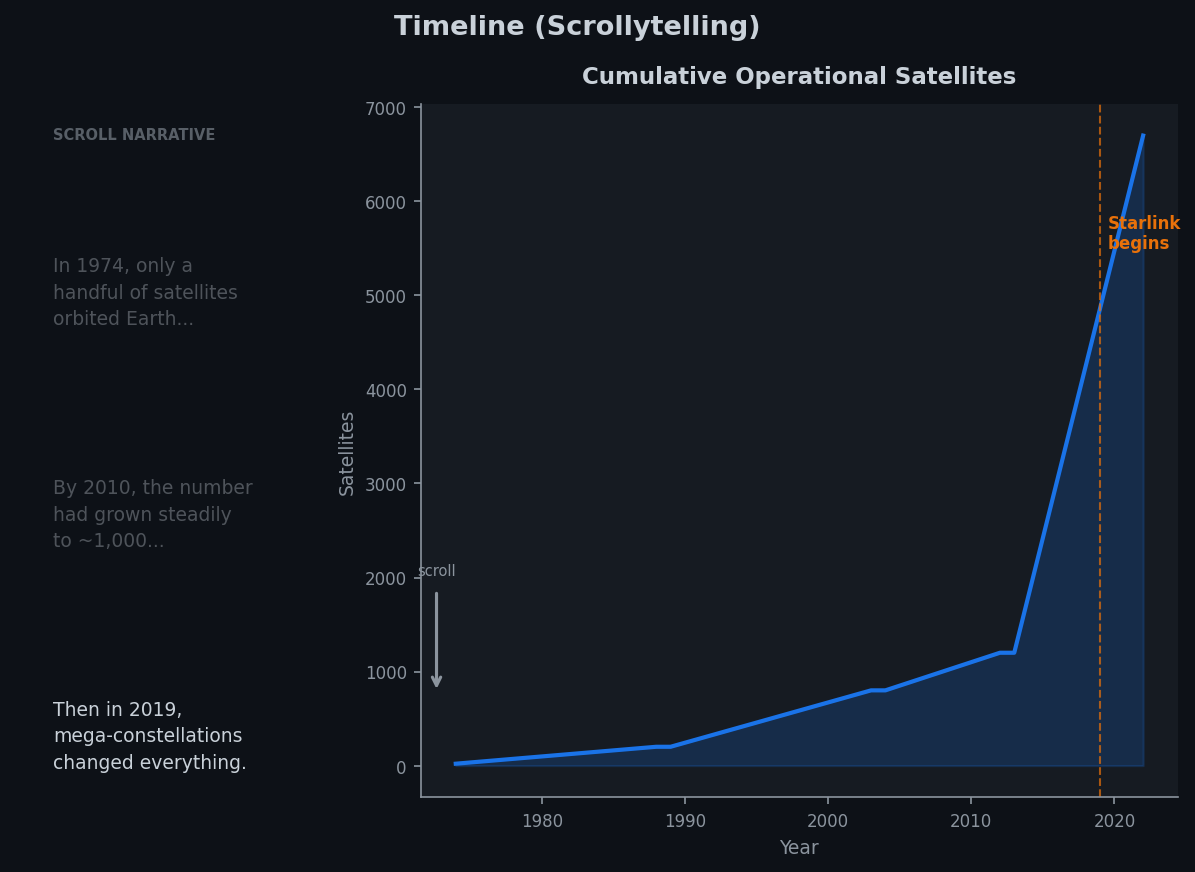
\includegraphics[width=0.95\textwidth]{01_timeline.png}
\end{minipage}\hfill%
\begin{minipage}[t]{0.46\textwidth}
\textbf{Wireframe 2 (M1).} Country bar + Lorenz curve in two columns. This sketch survives almost as drawn, with the Lorenz curve still annotated with the Gini 0.862 callout. What we added on top: a world choropleth as the geographic establishing shot above the row, an operator-deep-dive drawer beneath, and a country$\times$purpose specialization heatmap. The four pieces together answer the question the chapter title asks: \textit{who} owns space, \textit{how unequally}, \textit{which operators specifically}, and \textit{what for}.
\vspace{3pt}
\centering

\includegraphics[width=0.95\textwidth]{02_countries_lorenz.png}
\end{minipage}

\vspace{6pt}

\noindent
\begin{minipage}[t]{0.46\textwidth}
\textbf{Wireframe 3 (M1).} The 3D globe with a purpose$\times$orbit heatmap. This is the chapter that grew the most. The static globe became a Globe.gl viewport with three composed filters (orbit, year, mega-constellation) and a satellite-name search with a pulsing-ring spotlight. The heatmap stayed exactly as designed, because it was already doing what a heatmap should: making a 2D conditional distribution legible.
\vspace{3pt}
\centering

\includegraphics[width=0.95\textwidth]{03_globe_heatmap.png}
\end{minipage}\hfill%
\begin{minipage}[t]{0.46\textwidth}
\textbf{The piece that wasn't in M1.} A 3D hero. The original plan had the globe live only in Chapter 3, behind a paywall of scroll. The final site puts a separate Three.js scene at the top of the page: a textured Earth at the origin, all 6{,}713 satellites placed on their real inclined orbits (Kepler), animated with their physically-correct angular velocities, rendered through a custom GLSL sprite shader with bloom. The decision was driven by the screencast: a cinematic establishing shot in the first ten seconds lets us say more, faster, than any chart could. Chapter 4 (``The Next Decade'') was also added late: M1's narrative ended on present-day crowding, but the 2030 projections are what give the story stakes.
\vspace{3pt}
\centering
\shotplaceholder{Hero scene zoomed in: orbital cloud surrounding Earth}{0.95}
\end{minipage}

\newpage

% =====================================================================
% PAGE 3 — DATA & EXPLORATORY ANALYSIS
% =====================================================================

\eyebrow{03 \quad\textbullet\quad Data and exploratory analysis}\\[3pt]
{\Large\bfseries 6{,}713 satellites, cleaned and aggregated}

\vspace{6pt}

The dataset is the \href{https://www.kaggle.com/datasets/sujaykapadnis/every-known-satellite-orbiting-earth/data}{UCS Satellite Database} (Union of Concerned Scientists), snapshot 1 January 2023, with 27 attributes per satellite. Of the 6{,}718 raw rows, 5 are dropped during cleaning, leaving 6{,}713 satellites that the site ships with. The full data path lives in \texttt{scripts/build\_data.py} (about 700 lines, 23 unit + integration tests in \texttt{test\_build\_data.py}, all passing). Every transformation it applies is logged to \href{https://github.com/com-480-data-visualization/The-Outliers/blob/master/data/data_quality_flags.md}{\texttt{data/data\_quality\_flags.md}} so any reader can audit the decisions.

\vspace{2pt}

\subsection*{What the script does}

\textbf{Parses numerics.} Apogee, perigee, eccentricity, inclination, period. UCS ships these as strings with embedded commas; we coerce, drop rows where coercion fails on parameters we need.

\textbf{Reclassifies orbit class by physics, conservatively.} The UCS ``Class of Orbit'' column is the source of truth except where it is unambiguously contradicted by altitude or eccentricity: LEO/MEO satellites whose mean altitude is above 30{,}000 km override to GEO (catches Angosat-2 and WFOV Testbed), ``Elliptical'' satellites with near-zero eccentricity override to the right shell by altitude (catches Falconsat-7, Gaofen 11, Hisaki), and GEO satellites far from geostationary altitude with near-zero eccentricity drop back to LEO or MEO. We do not override satellites with genuinely moderate eccentricity, even when a naive threshold would flip them.

\textbf{Repairs eccentricity sign-error typos.} A handful of UCS rows record eccentricity outside $[0, 1)$ (for example \texttt{5.11E+02} instead of \texttt{5.11E-02}). We discard the bad value and recompute from perigee/apogee for classification, but log the original so it's traceable.

\textbf{Drops irrecoverable rows.} Five rows have either no inclination, no perigee \textit{and} no apogee, or perigee~$>$~apogee (a physical impossibility). These cannot be placed on the 3D globe and are excluded from both the aggregate counts and the per-satellite list so the two outputs always agree on the total.

\textbf{Normalizes operator names.} ``Spacex'' and ``SpaceX,'' ``Iridium Communications, Inc.'' and ``Iridium,'' a dozen others. We collapse them in a small lookup so the Chapter 2 operator chart isn't full of duplicates.

\textbf{Derives \texttt{constellation}.} Starlink, OneWeb, Iridium, Galileo are detected by case-insensitive name pattern (e.g.\ names starting with ``Starlink''). This drives the Chapter 3 mega-constellation isolator. Final distribution: Starlink 3{,}395, OneWeb 502, Iridium 73, Galileo 28, Other 2{,}715.

\vspace{2pt}

\subsection*{The picture that justified the entire project}

\noindent
\begin{minipage}[t]{0.48\textwidth}
\vspace{2pt}
A single histogram (right) explains why orbits cluster the way they do. The altitudes are not a smooth distribution: there are three sharp modes. LEO peaks around 500--600 km (Starlink at 550, Earth-observation sun-sync orbits at $\approx 700$). MEO peaks around 19{,}000--23{,}000 km (the Galileo, GLONASS and GPS navigation shells). GEO is a single spike at $\approx 36{,}000$ km (the geostationary belt). This trimodal structure is what makes the LEO/MEO/GEO/Elliptical buckets clean rather than arbitrary, and it's the structural foundation of every other chart in the site: the orbit donut, the heatmap, the time-slider history, the bloom-ringed shells in the hero.
\end{minipage}\hfill%
\begin{minipage}[t]{0.48\textwidth}
\vspace{0pt}
\shotplaceholder{Histogram: altitude (km, log scale) coloured by orbit class}{0.95}
\end{minipage}

\vspace{4pt}

\subsection*{Output schema}

The script writes two JSON files. \texttt{satellites.json} carries pre-aggregated statistics keyed by chart: \texttt{cumulative\_launches}, \texttt{cumulative\_purpose\_by\_year}, \texttt{top\_countries}, \texttt{country\_counts}, \texttt{country\_purpose\_matrix}, \texttt{orbit\_distribution}, \texttt{purpose\_breakdown}, \texttt{purpose\_by\_orbit}, \texttt{top\_operators}, \texttt{operator\_details}, \texttt{lorenz\_curve}. \texttt{satellites-globe.json} is the slim per-satellite list (name, country, orbit class, purpose, altitude, inclination, launch year, constellation) consumed by the 3D scene and Globe.gl. The \texttt{-{}-check} mode verifies the committed JSONs match what the script would currently emit, so a stale build cannot accidentally land.

\newpage

% =====================================================================
% PAGE 4 — DESIGNING THE NARRATIVE
% =====================================================================

\eyebrow{04 \quad\textbullet\quad Designing the narrative}\\[3pt]
{\Large\bfseries A four-chapter arc, Freytag inside}

\vspace{6pt}

The defining decision was to commit to a \textit{linear} reading experience and let interactivity bloom from inside it, rather than build a dashboard the user has to assemble in their head. The visual reference was The Pudding's scrollytelling, the structural reference was Freytag's pyramid (Lecture~12). The reader does not need a hypothesis or a query to engage. They scroll, and a story unfolds. They can pause anywhere to interact.

\vspace{2pt}

\subsection*{Freytag's pyramid mapped to chapters}

\begin{tabularx}{\textwidth}{@{} l l X @{}}
\toprule
\textbf{Phase} & \textbf{Chapter} & \textbf{What it does}\\
\midrule
Exposition       & Hero                    & A black space with three sequential lines of poster text (\textit{A frontier. Then, an avalanche. 6{,}713 and counting.}), then a radial-iris wipe reveals the 3D Earth surrounded by the satellite cloud. Sets the scene with a single image.\\
Rising action    & Chapter 1, The Explosion & Cumulative-launches timeline paced by five scroll steps (1974, 1998, 2018, 2021, 2023), then a stacked-area showing how Communications absorbed the entire post-2019 growth.\\
Climax           & Chapter 2, Who Owns Space? & The inequality reveal: USA owns two thirds, one company owns half, Gini $0.862$. World choropleth, country bars, Lorenz curve, top-10 operators with deep-dive, country$\times$purpose specialization heatmap.\\
Falling action   & Chapter 3, The Congestion & The reader is given the keys: 3D globe with composed filters (orbit, year, constellation), year-history playback, satellite name search with spotlight. The same 6{,}713 dots from the hero are now theirs to inspect.\\
Resolution       & Chapter 4, The Next Decade & 2023 vs.\ $\approx 2030$ filing totals. A 12$\times$ growth bar. Closes the arc without preaching.\\
\bottomrule
\end{tabularx}

\vspace{4pt}

\subsection*{Why these chart types, specifically}

\textbf{Area chart over a bar chart for the timeline} (L6, L11). Cumulative counts year-by-year are a continuous quantity; bars would imply discrete events. Area fills the space below the line, which gives the chapter its second visual finding: the area under the curve is mostly post-2019.

\textbf{Stacked area for purpose-over-time} (L4, L6). Showing six absolute counts on a shared X axis would clutter; a single stacked area reads as ``what the satellites were for, year by year'' at a glance. The order (Other at the bottom, Communications on top) is chosen so the blue Communications band sits where its post-2019 explosion is most visible.

\textbf{World choropleth for country distribution} (L8). The country bar chart ranks (which is what we want for an ``inequality'' chapter), but a map gives the geographic intuition that a list cannot. Equal Earth projection because Mercator would give Greenland and Antarctica visual weight they don't earn.

\textbf{Lorenz curve over a Pareto-style chart} (L6, L11). The Lorenz curve is the canonical inequality visualization, and the Gini coefficient is its single number. Pairing the curve with the 0.862 annotation makes the math legible without a stats degree.

\textbf{Country$\times$purpose heatmap over a stacked bar} (L6, L11). A heatmap shows \textit{specialization}, not just volume: the USA-Communications cell glows bright not because the USA has the most satellites, but because Communications is what it focuses on. A stacked bar would hide that pattern in the proportions.

\textbf{3D globe over a 2D world map} (L8). Real altitude matters for the orbit story. A 2D map projection erases altitude. Globe.gl gives us altitude, drag-rotate, and per-point hover with the right framing for the screencast.

\newpage

% =====================================================================
% PAGE 5 — VISUAL DESIGN DECISIONS
% =====================================================================

\eyebrow{05 \quad\textbullet\quad Visual design decisions}\\[3pt]
{\Large\bfseries A dark space, four hues, two typefaces}

\vspace{6pt}

The site is a single visual system. The same palette, type, and motion grammar runs from the hero through Chapter 4 and the stats bar. The goal was that any screenshot of the site should be recognizable as the same project, regardless of which chapter it comes from.

\vspace{2pt}

\subsection*{Color}

Four orbit-class hues form the spine: \textcolor{accentBlue}{\textbf{blue \#1A73E8}} for LEO, \textcolor{accentOrange}{\textbf{orange \#E8710A}} for MEO, \textcolor{accentGreen}{\textbf{green \#34A853}} for GEO, \textcolor{accentPurple}{\textbf{purple \#9334E6}} for Elliptical. The same hex codes are used identically in the D3 charts, the Three.js hero scene's GLSL shader, and the Chapter 3 globe.gl points layer, defined once in \texttt{prototype/js/charts/shared.js} and imported wherever a chart needs the palette. The dual role (orbit class \textit{and} accent / highlight) is the one place where the palette had to flex: in the country bar chart, the USA bar uses the orange accent because it is the dominant entry, which conflicts with MEO's orange. We accepted the conflict because the rule ``the dominant entry is orange'' generalizes cleanly across charts (it is also the highlight for active constellation isolator buttons), whereas a sixth color would have diluted the orbit-class palette.

\vspace{2pt}

\subsection*{Typography}

Two families. \textbf{Space Grotesk} (700, 800) for headings, big numbers, and any monospace-feeling moment (year readouts, KPI tiles, axis labels for the operator drawer). \textbf{Inter} (300, 400, 600) for everything else: body copy, captions, button labels, tooltips. Sizes step in a 1.25 modular scale. \texttt{tabular-nums} is on for any column of numbers that the reader will visually align.

\vspace{2pt}

\subsection*{Dark theme}

A black-to-near-black background (\texttt{\#000} body, \texttt{\#050508} for sections) is doing three things at once: it lets the 3D scene feel like real space without a black-rectangle frame, it gives the satellite-cloud bloom and the gradient charts maximum contrast, and it lowers the energy cost of a long-running animation on the user's screen. The risk is text legibility; we mitigate with the secondary text color (\texttt{\#9BA3B5}), generous line height (1.6 body, 1.7 chart steps), and an explicit \texttt{prefers-color-scheme} that doesn't fight the OS.

\vspace{2pt}

\subsection*{Motion}

Two principles, applied consistently. \textbf{(1) Motion is informative or it is gone.} Every transition either communicates state change (a constellation isolator button activating, a slider thumb moving, a country bar growing in on mount) or it is removed in \texttt{prefers-reduced-motion}. The hero intro acts, the cloud orbital motion, the chapter-entrance fades, and the Globe.gl autorotation are all gated on the same media query. \textbf{(2) Easing matches the cadence of reading.} The repeated curve \texttt{cubic-bezier(0.22, 1, 0.36, 1)} (a soft ease-out) is used for chart entrances, slider thumb scale, drawer slide, fade-in opacities, and Lenis smooth-scroll. The interval (350--850 ms) sits in the range where the eye registers the motion without waiting for it.

\vspace{2pt}

\subsection*{Library choices, with rationale}

\textbf{D3 v7} for every 2D chart. Familiar from the lectures (L4, L5), gives us full layout control, hooks into the existing palette tokens directly. We did not reach for higher-level chart libraries (Vega-Lite, Plotly) because the project's interaction model is non-standard (composed filters, linked views, a slide-in drawer) and we wanted no friction at the boundary.

\textbf{Globe.gl} for the Chapter 3 globe. It is a thin wrapper around three-globe / Three.js but with a clean declarative API (\texttt{pointsData}, \texttt{ringsData}, \texttt{pointOfView}), built-in atmosphere and texture loaders, and a working camera controller. Writing this from scratch in raw Three.js would have cost two days and shipped strictly worse.

\textbf{Three.js (r170) directly} for the hero scene, because we needed full control: per-vertex GLSL shader on the satellite cloud, real Kepler positions updated 60 times a second, a custom UnrealBloomPass composer, sRGB-correct output via \texttt{OutputPass}. We ship Three.js as an ES module from \texttt{esm.sh} so the post-processing example modules resolve their bare \texttt{"three"} imports to the same Three.js instance, avoiding the ``two Three.js'' class-identity bug that bit us during integration.

\textbf{TopoJSON + world-atlas} for the choropleth. 100 KB of vector geometry, decoded with \texttt{topojson-client}. We considered raster but the map needs hover hit-testing on every country.

\textbf{Lenis} for smooth scroll, \textbf{D3.js} for every other transition. We deliberately did not bring in GSAP. Lenis owns the scroll, IntersectionObserver drives the fade-ins, D3 transitions drive every chart entrance. The dependency surface stays small.

\textbf{Pre-aggregated JSON over in-browser CSV parsing}. \texttt{build\_data.py} ships two tight JSONs (about 200 KB combined, gzipped to about 40 KB). Parsing the 6{,}700-row UCS CSV on every page load would add hundreds of milliseconds to first paint and dump a megabyte over the wire. The build script is the right place for the aggregation, the per-chart shape, and the data-quality logging.

\newpage

% =====================================================================
% PAGE 6 — INTERACTIONS AND CHALLENGES
% =====================================================================

\eyebrow{06 \quad\textbullet\quad Interactions and challenges}\\[3pt]
{\Large\bfseries Six interactions, three problems that nearly bit us}

\vspace{6pt}

\subsection*{The interactions, in the order the reader meets them}

\textbf{1. Cinematic hero intro.} Three poster lines (``A frontier.'' $\to$ ``Then, an avalanche.'' $\to$ ``6{,}713 and counting.'') crossfade over a black vignette; a radial-iris wipe reveals the 3D scene; the CROWDED ORBIT title slides in. One-shot: latched after \texttt{final}, so scrolling back up does not replay it. The phase controller (\texttt{cinematic-hero.js}) is a tiny state machine driven by wheel/touch input that re-emits to the rest of the page only after the latch.

\textbf{2. Scrollytelling timeline (Chapter 1).} Native \texttt{IntersectionObserver}-style scroll handler dispatches a \texttt{scrolly-step} event when the active step changes; the area chart listens and updates a clip-path width plus an annotated marker. Five steps, five known years, deterministic.

\textbf{3. Operator deep-dive drawer (Chapter 2).} Click any of the top 10 operator bars and a 480 px panel slides in from the right with the operator's launch sparkline, orbit-class horizontal bars, purpose horizontal bars, and KPI tiles. Closeable via the {\sffamily $\times$} button, the dim scrim, or Escape. Body scroll is locked while open (\texttt{lenis.stop()}).

\textbf{4. Composed filters on the Chapter 3 globe.} Three independent filters apply at once: orbit-class buttons (LEO / MEO / GEO / Elliptical / All), mega-constellation isolator (Starlink / OneWeb / Iridium / Galileo / Other / All), and a year slider with a play-history sweep ($\approx 3$ years/sec). A single \texttt{applyFilters()} composes all three. Selecting a constellation also dispatches a \texttt{constellation-changed} event that the world map and the country bar chart subscribe to: the home country lights up on both, linked-view style (L5).

\textbf{5. Satellite name search with pulsing-ring spotlight.} Live filter over all 6{,}713 names. Ranking is prefix-match first, then shorter name, then lexicographic; so ``hubble'' surfaces the Hubble Space Telescope as the top hit, ``iss'' surfaces the ISS, ``star'' opens onto the Starlink fleet. Picking a result flies the Globe.gl camera to the satellite's position and \texttt{ringsData} pulses a white ring at that point's altitude.

\textbf{6. Future projection (Chapter 4).} A two-bar comparison on the same X scale (so the lengths are visually honest) with five colored segments for the projected 2030 fleet. A collapsed Sources block under the chart cites every filing source (FCC, ITU, UK Space Agency).

\vspace{3pt}

\subsection*{Challenges, with what we did about each}

\textbf{The two-Three.js bug.} Adding the hero's Three.js scene alongside Globe.gl initially crashed Globe.gl with \texttt{z0.Timer is not a constructor}. Globe.gl bundles its own Three.js internally, and our external Three.js (loaded as a UMD script tag) overrode \texttt{window.THREE} with an older version that lacked \texttt{THREE.Timer}. Fix: load the hero's Three.js as an ES module from \texttt{esm.sh} so it has its own isolated instance, never touches \texttt{window.THREE}, and Globe.gl keeps its own bundled copy. The two instances coexist without conflict.

\textbf{Rendering 6{,}713 animated satellites at 60 fps.} Naive Three.js (one \texttt{Mesh} per satellite) would have been a 6{,}700-draw-call disaster. We use a single \texttt{BufferGeometry} with one vertex per satellite, custom \texttt{ShaderMaterial} (vertex shader handles per-orbit point size and depth attenuation, fragment shader draws each as a soft glowing disk with additive blending), and a tight per-frame loop that updates only the \texttt{position} attribute. CPU cost is roughly 30 floating-point ops per satellite per frame ($\approx 200$~K total) and the GPU upload is $\approx 80$~KB per frame. Comfortable margin on a 2019 laptop.

\textbf{Operator-name normalization.} The UCS CSV writes ``Spacex,'' ``SpaceX,'' ``Space Exploration Technologies,'' and ``Space Exploration Technologies Corp.\ (SpaceX)'' for the same operator. We collapse those (and 17 others) in a static lookup table in \texttt{build\_data.py}. Without this, the top-10 operator chart would show three SpaceX entries.

\textbf{The Chapter 1 sticky-chart on tall content.} The scrollytelling chart uses \texttt{position: sticky} and \texttt{min-height: 300vh} on its container so the chart sticks for the full scroll height. When we added the second panel (purpose-over-time) inside the same chapter, the sticky rule applied to it too and created a giant dark gap. Tightening the selector to \texttt{:has(.scrolly)} scoped the rule to the right container only.

\newpage

% =====================================================================
% PAGE 7 — TECHNICAL IMPLEMENTATION
% =====================================================================

\eyebrow{07 \quad\textbullet\quad Technical implementation}\\[3pt]
{\Large\bfseries Build, ship, test}

\vspace{6pt}

\subsection*{Architecture}

The site is fully static. A Python build script transforms one CSV into two JSONs, the browser fetches them, every chart renders client-side. No backend, no build step on the client. The data pipeline is the only non-trivial moving part:

\vspace{3pt}
\begin{center}
{\small\ttfamily
UCS CSV $\longrightarrow$ build\_data.py $\longrightarrow$ satellites.json + satellites-globe.json $\longrightarrow$ fetch() $\longrightarrow$ D3 / Three.js / Globe.gl
}
\end{center}
\vspace{3pt}

The Python side enforces correctness (23 unit + integration tests, all green); the JS side stays dumb because the data shape is already right.

\subsection*{Module layout}

\texttt{prototype/js/} is organized into four buckets. \textbf{Charts} (\texttt{charts/*.js}, one file per chart) each export a top-level draw function and share constants from \texttt{shared.js} (palette, tooltip). \textbf{Scene} (\texttt{scene/journey.js}) is the hero's Three.js scene, loaded as an ES module with its own Three.js instance. \textbf{Effects} (\texttt{effects/stars.js}) are the page-wide canvas decorations. \textbf{Controllers}: \texttt{main.js} (boot), \texttt{globe.js} (Chapter 3 Globe.gl + filters + search), \texttt{scrollytelling.js} (Chapter 1 step observer), \texttt{scroll.js} (Lenis + chapter fade-ins), \texttt{nav.js} (chapter navigator), \texttt{cinematic-hero.js} (intro state machine).

Imports stay flat (no bundler, no transpiler). Two files are ES modules because they need ES imports (\texttt{scene/journey.js} for Three.js, \texttt{scroll.js} for Lenis); everything else is a plain global \texttt{<script>}, in deterministic load order, with \texttt{shared.js} first. This is intentional: the team can clone the repo, run a Python HTTP server, and edit any chart with no toolchain.

\subsection*{Build pipeline and testing}

\texttt{scripts/build\_data.py} owns the full transformation. \texttt{-{}-check} mode recomputes both JSONs in memory and compares against the committed files, exiting non-zero on drift. \texttt{scripts/test\_build\_data.py} runs 23 tests: orbit-classification rules, eccentricity-sign-error recovery, purpose normalization, operator-name normalization, sanity-check flagging, end-to-end build against the real CSV, JSON validity. The whole pipeline runs in about 1.5 seconds; the tests in $<$ 1 second.

\subsection*{Performance}

The site loads in $<$1.5 s first paint on a 4G connection. The two JSONs gzip to $\approx 40$ KB, Three.js is the largest dependency ($\approx 150$ KB gzipped, loaded as an ES module). The 6{,}713-satellite scene renders consistently at 60 fps on integrated-graphics laptops; we verified on a 2019 MacBook Air and a Windows-on-ARM Surface. The Chapter 3 Globe.gl viewport hovers around 55--60 fps depending on autorotate. \texttt{pointsMerge(true)} keeps the 6{,}713-point cloud as a single GPU mesh.

\subsection*{Accessibility}

Every interactive control (filter buttons, year slider, play button, search input, drawer close, constellation buttons) has an \texttt{aria-label} and is keyboard-reachable. The operator drawer is a real \texttt{role="dialog"} with \texttt{aria-modal} and focus management on open. Globe.gl content has an \texttt{aria-label} description of the visual so screen readers do not just see ``canvas.'' A \texttt{<noscript>} block tells JS-disabled visitors what they are missing and how to fix it. The whole site degrades under \texttt{prefers-reduced-motion}: Lenis is not constructed, fades land immediately, the hero's orbital motion and the globe's autorotation freeze. Color contrast on body text is $> 7$:$1$, on secondary text $> 4.5$:$1$.

\subsection*{Responsive}

Three breakpoints (700 px, 900 px, viewport-bound). The country bar / Lorenz / operator / heatmap row collapses to single-column under 900 px. The time-slider card stacks the play button above the track under 700 px. The operator drawer takes 100 vw on phones. The 3D globe and the hero scene scale via \texttt{ResizeObserver} on their containers, not on window resize, so late-arriving layout (fonts loading, scrollbar appearing) does not leave them at 0 px wide.

\subsection*{Browser support}

Tested on Chrome, Firefox, Safari (desktop and iOS), Edge. The CSS uses \texttt{:has()} for one selector (Chapter 1 sticky scoping), which lands in every major browser shipped since late 2023. Earlier browsers see a static, non-immersive version of the site that still works because every chart degrades gracefully without the JS post-processing.

\newpage

% =====================================================================
% PAGE 8 — PEER ASSESSMENT + REFLECTION
% =====================================================================

\eyebrow{08 \quad\textbullet\quad Peer assessment and reflection}\\[3pt]
{\Large\bfseries Who did what, and what we would do differently}

\vspace{6pt}

The contributions below reflect the actual commit history and pairing during the working sessions of milestone 3. Every member contributed across the stack; the breakdown captures where each took primary ownership.

\vspace{2pt}

\renewcommand{\arraystretch}{1.18}
\begin{tabularx}{\textwidth}{@{} l X r @{}}
\toprule
\textbf{Member} & \textbf{Primary contributions} & \textbf{Share}\\
\midrule
\textbf{Kevin Abou Jaoude} \newline (358300)
& Data pipeline expansion in \texttt{build\_data.py}: new aggregations for cumulative-purpose-by-year, country counts, country$\times$purpose matrix, operator deep-dive details, plus the constellation and launch-year fields on the per-satellite list (23 tests passing throughout). Chapter 4 (``The Next Decade'') projection chart with the citation block. Lenis smooth-scroll integration and the chapter-entrance fade-in observer. Site-wide accessibility pass (\texttt{aria-label}s, \texttt{noscript} fallback, \texttt{prefers-reduced-motion} guards, Open Graph meta). Repo hygiene: README v2, MIT \texttt{LICENSE}, expanded \texttt{.gitignore}. Process-book authoring and structure. & 1/3\\
\addlinespace[2pt]
\textbf{Youssef Dib} \newline (339964)
& Cinematic hero intro: three-act poster sequence, radial-iris vignette wipe, latched phase state machine that consumes wheel/touch input without leaking page scroll. Fixed top-right chapter navigator (open / close / active-chapter tracking via IntersectionObserver). Hero 3D scene polish: \texttt{UnrealBloomPass} post-processing, custom GLSL shader for soft-glow satellite sprites, orbit-class color tuning so each colored shell reads against the LEO mass. Globe.gl robustness: Ctrl-to-zoom gating with on-screen hint, \texttt{ResizeObserver} pattern, atmosphere alpha fix, scrollbar hiding so the layout never shifts. & 1/3\\
\addlinespace[2pt]
\textbf{Mark Nabbout} \newline (358312)
& Chapter 1 stacked area chart (purpose over time) with the post-2019 Starlink-era annotation. Chapter 2 world choropleth (D3 + TopoJSON, Equal Earth, log color scale, country-name mapping). Chapter 2 country$\times$purpose specialization heatmap with floating info card. Chapter 2 top-operators bar chart and full deep-dive drawer (launch-timeline sparkline, orbit and purpose mini-bars, KPI tiles, focus-trapped \texttt{role="dialog"}). Chapter 3 year-filter slider with play-history sweep, mega-constellation isolator with linked-view dispatch, satellite name search with pulsing-ring spotlight. Linked-country highlighting wiring across the world map and the country bar chart. & 1/3\\
\bottomrule
\end{tabularx}

\vspace{6pt}

\subsection*{What surprised us}

\textbf{The data was less linear than expected.} M1 framed the story as ``orbit is filling up.'' That's true, but the Chapter 1 stacked area showed something sharper that we did not anticipate: it is filling up \textit{with one purpose}. Communications was already 40\% of the fleet in 2018; by 2022 it was 72\%. The chapter changed shape because we found that finding.

\textbf{Performance was not the bottleneck.} We expected 6{,}713 animated satellites at 60 fps to be a fight. The custom shader handled it on the first try because the GPU is doing exactly the thing it is good at (one vertex per satellite, one position update per frame, additive-blended quad sprites). The bottlenecks we actually hit were CDN-related: a Lenis URL that 404'd silently, a Three.js post-processing module trying to bare-import \texttt{"three"} without an import map.

\textbf{Honest data caveats land harder than we feared.} We worried that the Chapter 4 ``filings are not deployments'' caveat would deflate the punch of the 12$\times$ headline. It didn't. Putting the citations in a collapsed expandable block, with a single warning line about deployment slippage, came off as confident rather than hedging.

\vspace{2pt}

\subsection*{What we would do differently with more time}

\textbf{Real ephemeris.} Our 3D scene places satellites on inclination-bounded \textit{visual} positions, not their real lat/lng at a given instant. With real two-line-element data from CelesTrak, the hero scene could show satellites where they actually are right now. The cost is a recurring data fetch and a satellite.js dependency. Worth doing as a v2.

\textbf{A debris and conjunction layer.} The story stops at active satellites. The full story includes the $\approx 30{,}000$ tracked debris objects and a Kessler-syndrome explainer. That is its own chapter and its own dataset (NORAD), but the same machinery would carry it.

\textbf{A guided auto-tour mode.} A play button at the top of the page that scripts a camera flythrough across all four chapters, so a first-time visitor with no idea what scrollytelling is gets the entire story in 90 seconds without scrolling. Effectively the screencast, but built into the page.

\textbf{Localization.} The narrative is in English. Translations would not change the data; they would change the audience. Most of the strings live in one HTML file, so this is engineering, not research.

\textbf{Sound.} A subtle ambient layer with a mute toggle, off by default. Risky to do well, immediate to do badly. We chose to do nothing rather than do it half-way; with more time we'd try it.

\vspace{4pt}

\begin{center}
{\footnotesize\color{textSec}Crowded Orbit \quad\textbullet\quad COM-480 \quad\textbullet\quad EPFL Spring 2026}\\
{\footnotesize\color{textSec}\url{https://com-480-data-visualization.github.io/The-Outliers/}}
\end{center}

\end{document}
